\section{Estimación de parámetros}\label{sec:estimacion-results}

En todos los resultados presentados se utiliza \(\Delta t = 1 \text{día}\). Se probó con valores más pequeños sin alterar el desempeño del método.

%\subsection{Modelo con una clase}
\subsection{Modelo multiclase con datos sintéticos} \label{subsec:sintetico}

Se ...

Se utilizan los datos de movilidad de dos comunas (...) para generar las matrices de tiempos de residencia variables en el tiempo. Se fijan valores \(\gamma_E = 1/5.1, \gamma_I = 1/8.2\) y condiciones iniciales... Se fija riesgos \(\beta_{\text{hogar}} = 1\) y \(\beta_{\text{exterior}} = 1.88\). 

Mediante prueba y error se genera controles (diferentes) para cada clase, de forma que el total de casos acumulados tengan órdenes de magnitud similares a los datos reales.

A partir de la solución de la ecuación diferencial es posible obtener las series \(C_1, C_2\). Las observaciones son obtenidas con \(\Delta t = 1\) [día]. Se utilizan estas observaciones directamente (sin añadir ruido), y el filtro asume que tienen un ruido pequeño (G = diag(10)...). 

Se suponen condiciones iniciales diferentes a las utilizadas en la solución (...), y se eligen matrices de covarianza de tal forma de obtener resultados razonables. Un ejemplo de las estimaciones de estado obtenidas puede verse en la figura \ref{synth-all-nohigh}.



\begin{figure}[!h]
\centering
\includegraphics[width=0.99\textwidth]{img/resultados/synth/kalman_grouped_allstates_allgroups\parameterstring}
\caption{Ejemplo de estimación de estados y parámetros variables en el tiempo con \textit{Kalman Smoother}, a partir de las observaciones del número de casos acumulados \(C_1, C_2\).}
\label{synth-all-nohigh}
\end{figure}

Las matrices de covarianza iniciales son elegidas de modo tal que las soluciones reales quedan a una desviación estándar de la estimación, como se ve en la figura \ref{synth-e-comp-high}.


\begin{figure}[!h]
     \centering
     \begin{subfigure}[b]{\textwidth}
         \centering
         \includegraphics[width=.8\textwidth]{img/resultados/synth/kalman_grouped_E_high1\parameterstring}
         \caption{Clase \(1\).}
     \end{subfigure}
     \hfill
     \begin{subfigure}[b]{\textwidth}
         \centering
         \includegraphics[width=0.8\textwidth]{img/resultados/synth/kalman_grouped_E_high2\parameterstring}
         \caption{Clase \(2\).}
     \end{subfigure}
        \caption{Casos Expuestos, comparando resultados obtenidos con solución real, en valores absolutos y normalizados con respecto a la cantidad de personas por clase.}
        \label{synth-e-comp-high}
\end{figure}


Como se ve en la figura \ref{synth-alpha-comp-high}, es posible estimar el factor sanitario a partir de los datos, con ciertas consideraciones. En las secciones siguientes  se hablará en más detalle de la sensibilidad de la estimación con respecto a los parámetros del filtro. Más específicamente, se estudia la sensibilidad de la estimación del factor sanitario con respecto al parámetro \(\beta_{\text{exterior}}\) y la condición inicial. Se recuerda que se hizo la simplificación de que los ruidos en la dinámica son independientes, es decir que el ruido está dado por una matriz normal multivariada con matriz de covarianzas diagonal. Nos interesa por tanto, solo la diagonal de la matriz, las varianzas. Se muestra el efecto en la estimación al usar distintos valores para la matriz de varianzas.

\begin{figure}[!h]
     \centering
     \begin{subfigure}[b]{\textwidth}
         \centering
         \includegraphics[width=.99\textwidth]{img/resultados/synth/kalman_grouped_alpha_high1\parameterstring}
         \caption{Clase \(1\).}
     \end{subfigure}
     \hfill
     \begin{subfigure}[b]{\textwidth}
         \centering
         \includegraphics[width=0.99\textwidth]{img/resultados/synth/kalman_grouped_alpha_high2\parameterstring}
         \caption{Clase \(2\).}
     \end{subfigure}
        \caption[Factor sanitario, caso sintético]{Factor sanitario, comparando resultados obtenidos con función de control usada para general los datos, acotando el dominio en el eje \(y\) para mejor apreciación.}
        \label{synth-alpha-comp-high}
\end{figure}


\subsection{Sensibilidad con respecto a \(\beta_{\text{exterior}}\) y \(\alpha_0\)} \label{subsec:sensibeta}

\begin{figure}[H]
\centering
\begin{subfigure}[b]{0.47\textwidth}
     \centering
     \includegraphics[width=\textwidth]{img/resultados/synth/\stringsensiparam_high1_\stringrealandcovsparam\stringparamtwo.pdf}
     \caption{Estimación control clase 1, suponiendo conocidos \(\gamma_E = 1/5.1\) y \(\gamma_I = 1/7.2\)}
     \label{fig:legend-sensi-b-class1-gamma_real}
\end{subfigure} 
\hfill
\begin{subfigure}[b]{0.47\textwidth}
     \centering
     \includegraphics[width=\textwidth]{img/resultados/synth/\stringsensiparam_high2_\stringrealandcovsparam\stringparamtwo.pdf}
     \caption{Estimación control clase 2,  suponiendo conocidos \(\gamma_E = 1/5.1\) y \(\gamma_I = 1/7.2\)}
     \label{fig:legend-sensi-b-class2-gamma_real}
\end{subfigure} 
\hfill
\begin{subfigure}[b]{0.47\textwidth}
     \centering
     \includegraphics[width=\textwidth]{img/resultados/synth/\stringsensiparam_high1_\stringrealandcovsparam\stringparamthree.pdf}
     \caption{Estimación control clase 1,  con \(\gamma_E = 1/5.8\) y \(\gamma_I = 1/8.2\)}
     \label{fig:legend-sensi-b-class1-gamma_estimado}
\end{subfigure} 
\hfill
\begin{subfigure}[b]{0.47\textwidth}
     \centering
     \includegraphics[width=\textwidth]{img/resultados/synth/\stringsensiparam_high2_\stringrealandcovsparam\stringparamthree.pdf}
     \caption{Estimación control clase 2,  con \(\gamma_E = 1/5.8\) y \(\gamma_I = 1/8.2\)}
     \label{fig:legend-sensi-b-class2-gamma_estimado}
\end{subfigure} 
\hfill
\begin{subfigure}[b]{0.75\textwidth}
 \centering
\scalebox{0.7}{
\begin{tikzpicture}
	\begin{pgfonlayer}{nodelayer}
		\node [style=none] (0) at (-0.5, 1.25) {};
		\node [style=none] (1) at (1, 1.25) {};
		\node [style=none] (2) at (-0.5, 0.75) {};
		\node [style=none] (3) at (1, 0.75) {};
		\node [style=none] (4) at (-0.5, 0.25) {};
		\node [style=none] (5) at (1, 0.25) {};
		\node [style=none] (6) at (-0.5, -0.25) {};
		\node [style=none] (7) at (1, -0.25) {};
		\node [style=none] (8) at (1.5, 1.25) {$0.15$};
		\node [style=none] (9) at (1.5, 0.75) {};
		\node [style=none] (10) at (1.5, 0.75) {};
		\node [style=none] (11) at (1.5, 0.75) {$0.25$};
		\node [style=none] (12) at (1.5, 0.25) {};
		\node [style=none] (13) at (1.5, 0.25) {$0.35$};
		\node [style=none] (15) at (1.5, -0.25) {$0.45$};
		\node [style=none] (17) at (0.5, 1.75) {Condición inicial $\alpha_0$};
		\node [style=none] (19) at (12.5, 2.5) {$\beta_{\textrm{ext}}$};
		\node [style=none] (21) at (6.5, 1) {$\beta_{\text{ext}}$ solución real};
		\node [style=none] (22) at (5.5, 0.5) {};
		\node [style=none] (23) at (7, 0.5) {};
		\node [style=none] (24) at (7.5, 0.5) {};
		\node [style=none] (25) at (7.5, 0.5) {$1.88$};
		\node [style=none] (26) at (11.5, 2) {};
		\node [style=none] (27) at (13, 2) {};
		\node [style=none] (28) at (11.5, 1.5) {};
		\node [style=none] (29) at (13, 1.5) {};
		\node [style=none] (30) at (11.5, 1) {};
		\node [style=none] (31) at (13, 1) {};
		\node [style=none] (32) at (11.5, 0.5) {};
		\node [style=none] (33) at (13, 0.5) {};
		\node [style=none] (34) at (11.5, 0) {};
		\node [style=none] (35) at (13, 0) {};
		\node [style=none] (36) at (11.5, -0.5) {};
		\node [style=none] (37) at (13, -0.5) {};
		\node [style=none] (38) at (11.5, -1) {};
		\node [style=none] (39) at (13, -1) {};
		\node [style=none] (40) at (11.5, -1.5) {};
		\node [style=none] (41) at (13, -1.5) {};
		\node [style=none] (42) at (13.5, 2) {$1.2$};
		\node [style=none] (43) at (13.5, 1.5) {$1.5$};
		\node [style=none] (44) at (13.5, 1) {$1.8$};
		\node [style=none] (45) at (13.5, 0.5) {$2.1$};
		\node [style=none] (46) at (13.5, 0) {$2.4$};
		\node [style=none] (47) at (13.5, -0.5) {$2.7$};
		\node [style=none] (48) at (13.5, -1) {$3.0$};
		\node [style=none] (49) at (13.5, -1.5) {$3.3$};
	\end{pgfonlayer}
	\begin{pgfonlayer}{edgelayer}
		\draw [style={a0_1}] (0.center) to (1.center);
		\draw [style={a0_2}] (2.center) to (3.center);
		\draw [style={a0_3}] (4.center) to (5.center);
		\draw [style={a0_4}] (6.center) to (7.center);
		\draw [style=real] (22.center) to (23.center);
		\draw [style=beta1] (26.center) to (27.center);
		\draw [style=beta2] (28.center) to (29.center);
		\draw [style=beta3] (30.center) to (31.center);
		\draw [style=beta4] (32.center) to (33.center);
		\draw [style=beta5] (34.center) to (35.center);
		\draw [style=beta6] (36.center) to (37.center);
		\draw [style=beta7] (38.center) to (39.center);
		\draw [style=beta8] (40.center) to (41.center);
	\end{pgfonlayer}
\end{tikzpicture}
}
\end{subfigure}

\caption[Sensibilidad ante riesgo exterior y condición inicial del factor sanitario.]{Sensibilidad ante riesgo exterior y condición inicial del factor sanitario. Cada color representa un condición inicial diferente usada en la estimación, mientras que la opacidad de la solución representa la distancia de \(\beta_{\text{exterior}}\) al valor real; a mayor transparencia, más lejano.} \label{fig:legend-sensi-b}
\end{figure}

Los riesgos \(\beta \), las tasas \(\gamma_E\) y \(\gamma_I\), así como las condiciones iniciales, serán valores desconocidos en la práctica. Esta sección estudia el efecto de estos valores en la solución estimada. 

% gamma_e_real = 1/5.1; gamma_i_real = 1/7.2; beta_exterior_real = 1.88; 
Utilizando el caso sintético ya presentado, se estudia el efecto del valor \(\beta_{\text{exterior}}\) y de las condiciones iniciales para factor sanitario \(\alpha\) en los resultados. Los datos de casos acumulados observados fueron generados con un control conocido (línea verde) y parámetros \(\gamma_E = 1/5.1 [\text{días}]^{-1}\), \(\gamma_I = 1/7.2 [\text{días}]^{-1}\) y \(\beta_{\text{exterior}} = 1.88\).

Para distintos valores de \(\beta_{\text{exterior}}\) y distintas condiciones iniciales para el factor sanitario, se estima el factor sanitario suavizado a lo largo del tiempo y se compara con el valor de control usado para generar los datos. Los resultados pueden verse en la figura \ref{fig:legend-sensi-b}. Se estudian dos casos; uno con tasas de incubación \(\gamma_E\) y de remoción \(\gamma_I\) son conocidos (figuras \ref{fig:legend-sensi-b-class1-gamma_real} y \ref{fig:legend-sensi-b-class2-gamma_real}) y otro donde se utilizan valores pausibles para ambos parámetros (figuras \ref{fig:legend-sensi-b-class1-gamma_estimado} y \ref{fig:legend-sensi-b-class2-gamma_estimado}).

Se observa que tras una cierta cantidad de tiempo (\(t \geq 50\) la condición inicial es irrelevante y todas las soluciones dadas por un mismo \(\beta_{\text{exterior}}\) siguen la misma trayectoria. Al comenzar en una condición inicial demasiado baja, como \(\alpha_0 = 0.15\), se observa una tendencia a sobrecorregir el error antes de llegar a la trayectoria común. 

Para \(t \geq 200\), la estimación es menos exacta. Esto ya era visible en la figura \ref{synth-alpha-comp-high}, y probablemente se debe al hecho de que en este caso particular, para ese tiempo \(S_i(t) \approx 0\), así que la solución ya no es sensible al parámetro \(\alpha_i\).

Cuando los parámetros \(\gamma_E\) y \(\gamma_I\) son conocidos, la estimación del factor sanitario es más certera al usar un valor \(\beta_{\text{exterior}}\) más cercano al real. Esto se observa en la figuras \ref{fig:legend-sensi-b-class1-gamma_real} y \ref{fig:legend-sensi-b-class2-gamma_real}, donde las estimaciones más oscuras están justo en la línea verde que marca el factor sanitario de control usado para generar los datos.

En el caso en que los parámetros \(\gamma_E\) y \(\gamma_I\) son desconocidos y solo se usan valores pausibles, la estimación es menos exacata; el factor sanitario (para este caso particular) es subestimado al usar \(\beta_{\text{exterior}} = 1.8\), el más cercano al real (\(1.88\)) de entre los utilizados. Esto se observa en la figuras \ref{fig:legend-sensi-b-class1-gamma_estimado} y \ref{fig:legend-sensi-b-class2-gamma_estimado}, donde las estimaciones más oscuras están por debajo de la línea verde del factor sanitario de control.


% Conclusión del análisis de sensibilidad. 
Mientras la hipótesis \(\gamma_{Ei} = \gamma_E\) y \(\gamma_{Ii} = \gamma_I\) sea válida, es decir, que las tasas de incubación y remoción son iguales en cada clase, se puede esperar que las estimaciones del factor sanitario \(\alpha_i\) conserven la proporción entre ellas, de forma que, aunque no sean exactas, sí sea posible hacer afirmaciones del tipo ``la clase \(1\) enfrentó un 20\% más de riesgo que la clase \(2\) en este período de tiempo''. Si esto falla, entonces no se puede esperar que los factores sanitarios se expandan o contraigan uniformemenmte.


%gamma_e_real = 1/5.1; gamma_i_real = 1/7.2; beta_exterior_real = 1.88; 

%gamma_e = 1/5.8 ; gamma_i = 1/8.2; beta_exterior = 2.



%\subsection{Sensibilidad ante los parámetros \(\gamma_E, \gamma_I\)} \label{subsec:sensigamma}

\subsection{Sensibilidad ante la covarianza} \label{subsec:sensicov}
% 20. .^ collect(-2:0.4:0)
\begin{figure}[H]
\centering
\begin{subfigure}[b]{0.47\textwidth}
     \centering
     %\includegraphics[width=\textwidth]{img/resultados/synth/sensialphacov_alphacov0-003\stringsensiacov\stringparamfour.pdf}
     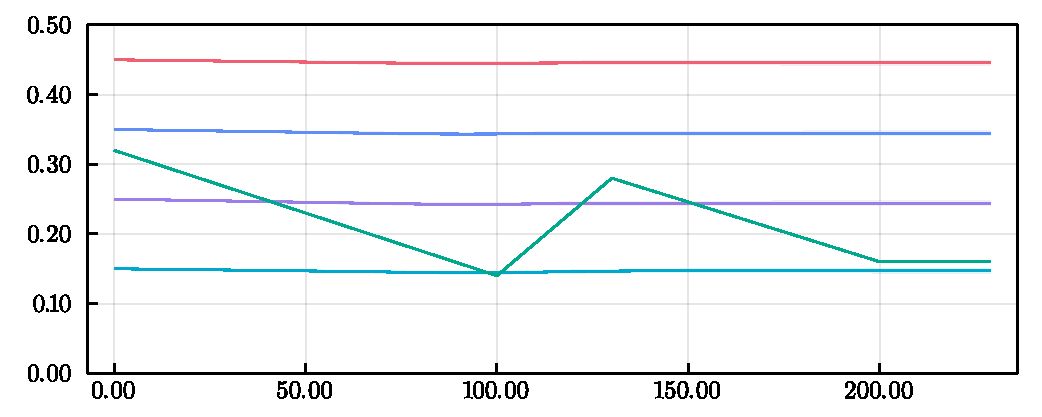
\includegraphics[width=\textwidth]{img/resultados/synth/sensialphacov_alphacov0-003_0alphaini0-15_0-1_0-45_high1_b2real1-88_gereal0-1961_gireal0-1389_acov0-8_aini0-27675_gcov0-05gamma_e_0-1961_gamma_i_0-1389_beta_2_1-8800.pdf}
     \caption{Estimación control clase 1, usando varianza para \(\alpha\) \(20^{-2.0}\)}
     \label{fig:legend-sensi-acov-class1--a}
\end{subfigure} 
\hfill
\begin{subfigure}[b]{0.47\textwidth}
     \centering
     %\includegraphics[width=\textwidth]{img/resultados/synth/sensialphacov_alphacov0-008\stringsensiacov\stringparamfour.pdf}
     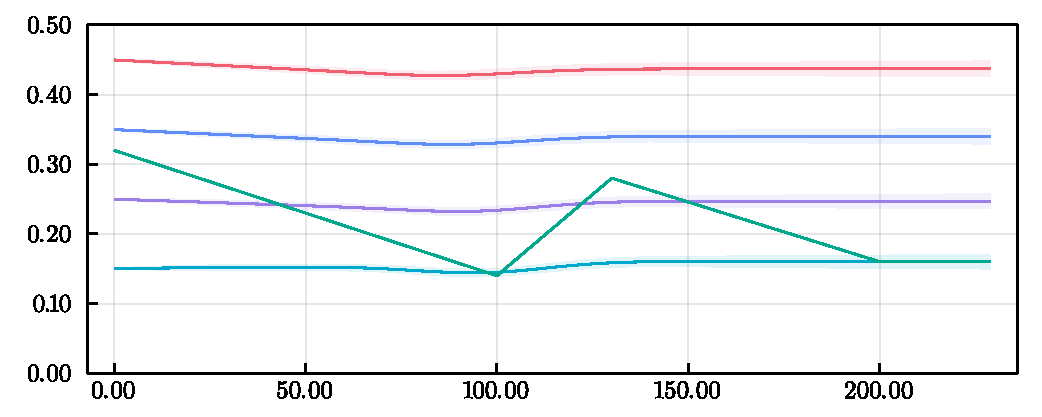
\includegraphics[width=\textwidth]{img/resultados/synth/sensialphacov_alphacov0-008_0alphaini0-15_0-1_0-45_high1_b2real1-88_gereal0-1961_gireal0-1389_acov0-8_aini0-27675_gcov0-05gamma_e_0-1961_gamma_i_0-1389_beta_2_1-8800.pdf}
     \caption{Estimación control clase 1, usando varianza para \(\alpha\) \(20^{-1.6}\)}
     \label{fig:legend-sensi-acov-class1--b}
\end{subfigure} 
\hfill
\begin{subfigure}[b]{0.47\textwidth}
     \centering
     %\includegraphics[width=\textwidth]{img/resultados/synth/sensialphacov_alphacov0-027\stringsensiacov\stringparamfour.pdf}
     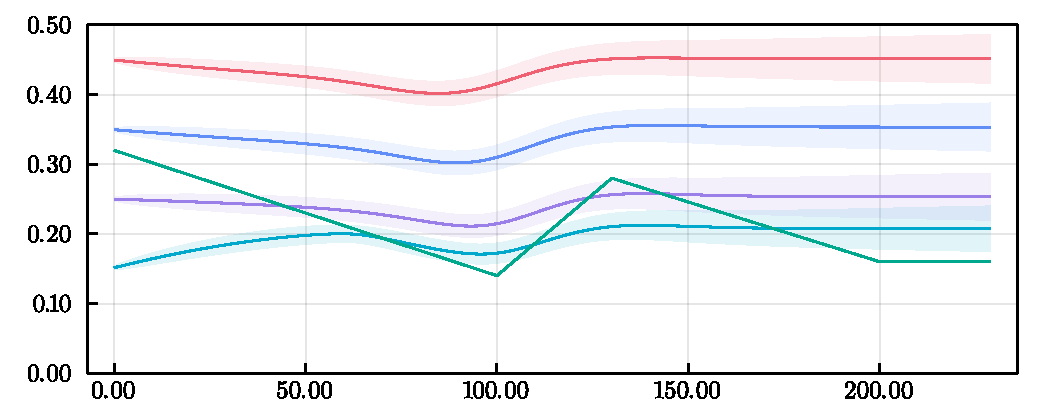
\includegraphics[width=\textwidth]{img/resultados/synth/sensialphacov_alphacov0-027_0alphaini0-15_0-1_0-45_high1_b2real1-88_gereal0-1961_gireal0-1389_acov0-8_aini0-27675_gcov0-05gamma_e_0-1961_gamma_i_0-1389_beta_2_1-8800.pdf}
     \caption{Estimación control clase 1, usando varianza para \(\alpha\) \(20^{-1.2}\)}
     \label{fig:legend-sensi-acov-class1--c}
\end{subfigure} 
\hfill
\begin{subfigure}[b]{0.47\textwidth}
     \centering
     %\includegraphics[width=\textwidth]{img/resultados/synth/sensialphacov_alphacov0-091\stringsensiacov\stringparamfour.pdf}
     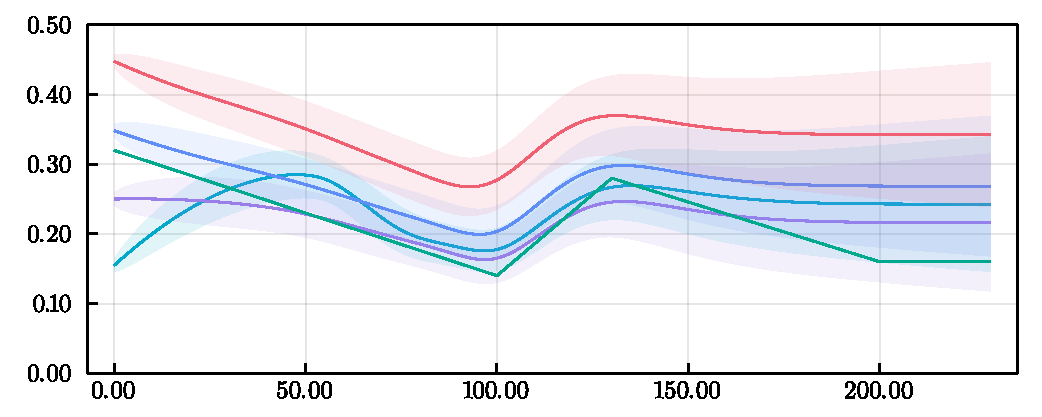
\includegraphics[width=\textwidth]{img/resultados/synth/sensialphacov_alphacov0-091_0alphaini0-15_0-1_0-45_high1_b2real1-88_gereal0-1961_gireal0-1389_acov0-8_aini0-27675_gcov0-05gamma_e_0-1961_gamma_i_0-1389_beta_2_1-8800.pdf}
     \caption{Estimación control clase 1, usando varianza para \(\alpha\) \(20^{-0.8}\)}
     \label{fig:legend-sensi-acov-class1--d}
\end{subfigure} 
\hfill
\begin{subfigure}[b]{0.47\textwidth}
     \centering
     %\includegraphics[width=\textwidth]{img/resultados/synth/sensialphacov_alphacov0-302\stringsensiacov\stringparamfour.pdf}
     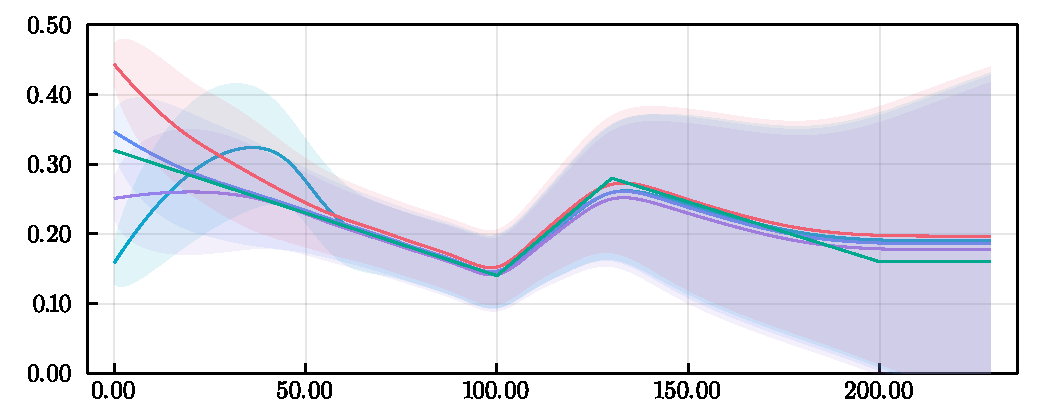
\includegraphics[width=\textwidth]{img/resultados/synth/sensialphacov_alphacov0-302_0alphaini0-15_0-1_0-45_high1_b2real1-88_gereal0-1961_gireal0-1389_acov0-8_aini0-27675_gcov0-05gamma_e_0-1961_gamma_i_0-1389_beta_2_1-8800.pdf}
     \caption{Estimación control clase 1, usando varianza para \(\alpha\) \(20^{-0.4}\)}
     \label{fig:legend-sensi-acov-class1--e}
\end{subfigure} 
\hfill
\begin{subfigure}[b]{0.47\textwidth}
     \centering
     %\includegraphics[width=\textwidth]{img/resultados/synth/sensialphacov_alphacov1-000\stringsensiacov\stringparamfour.pdf}
     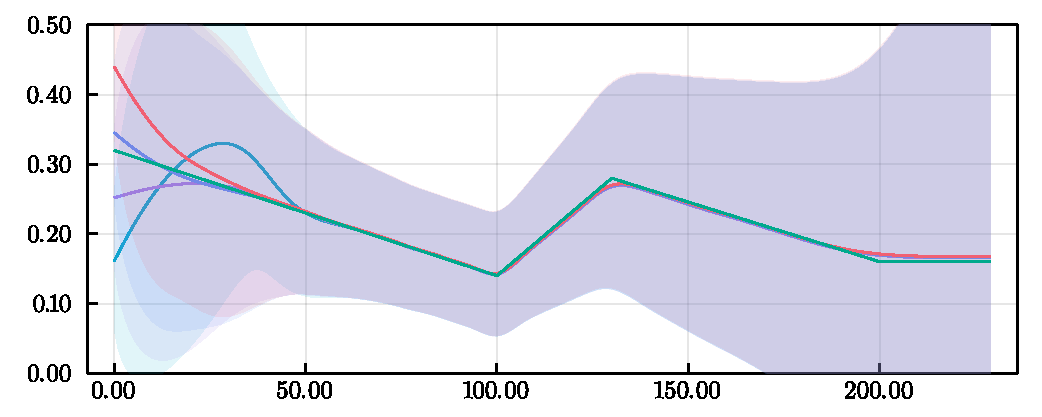
\includegraphics[width=\textwidth]{img/resultados/synth/sensialphacov_alphacov1-000_0alphaini0-15_0-1_0-45_high1_b2real1-88_gereal0-1961_gireal0-1389_acov0-8_aini0-27675_gcov0-05gamma_e_0-1961_gamma_i_0-1389_beta_2_1-8800.pdf}
     \caption{Estimación control clase 1, usando varianza para \(\alpha\) \(20^{0.0}\)}
     \label{fig:legend-sensi-acov-class1--f}
\end{subfigure} 
\hfill
\begin{subfigure}[b]{0.75\textwidth}
 \centering
\scalebox{0.7}{
\begin{tikzpicture}
	\begin{pgfonlayer}{nodelayer}
		\node [style=none] (0) at (-0.5, 1.25) {};
		\node [style=none] (1) at (1, 1.25) {};
		\node [style=none] (2) at (-0.5, 0.75) {};
		\node [style=none] (3) at (1, 0.75) {};
		\node [style=none] (4) at (-0.5, 0.25) {};
		\node [style=none] (5) at (1, 0.25) {};
		\node [style=none] (6) at (-0.5, -0.25) {};
		\node [style=none] (7) at (1, -0.25) {};
		\node [style=none] (8) at (1.5, 1.25) {$0.15$};
		\node [style=none] (9) at (1.5, 0.75) {};
		\node [style=none] (10) at (1.5, 0.75) {};
		\node [style=none] (11) at (1.5, 0.75) {$0.25$};
		\node [style=none] (12) at (1.5, 0.25) {};
		\node [style=none] (13) at (1.5, 0.25) {$0.35$};
		\node [style=none] (15) at (1.5, -0.25) {$0.45$};
		\node [style=none] (17) at (0.5, 1.75) {Condición inicial $\alpha_0$};
		\node [style=none] (21) at (6.5, 1) {};
		\node [style=none] (22) at (5.5, 0.5) {};
		\node [style=none] (23) at (7, 0.5) {};
		\node [style=none] (24) at (7.5, 0.5) {};
		\node [style=none] (25) at (7.5, 0.5) {Solución real};
	\end{pgfonlayer}
	\begin{pgfonlayer}{edgelayer}
		\draw [style={a0_1}] (0.center) to (1.center);
		\draw [style={a0_2}] (2.center) to (3.center);
		\draw [style={a0_3}] (4.center) to (5.center);
		\draw [style={a0_4}] (6.center) to (7.center);
		\draw [style=real] (22.center) to (23.center);
	\end{pgfonlayer}
\end{tikzpicture}
}
\end{subfigure}
\caption[Sensibilidad ante la varianza y condición inicial del factor sanitario.]{Sensibilidad ante la varianza y condición inicial del factor sanitario. Cada color representa una condición inicial diferente usada en la estimación.} \label{fig:legend-sensi-alphacov}
\end{figure}

Se recuerda que se hizo la simplificación de que los ruidos en la dinámica son independientes, es decir que el ruido está dado por una matriz normal multivariada con matriz de covarianzas diagonal. Nos interesa por tanto, solo la diagonal de la matriz, las varianzas. Se muestra el efecto en la estimación al usar distintos valores para la matriz de varianzas.

La figura \ref{fig:legend-sensi-alphacov} muestra la estimación del factor sanitario para distintos valores de varianza del ruido en la dinámica de este. Este valor refleja la certeza que tenemos en la dinámica del estado; si hay mucha, se usa una varianza baja. Si no hay tanta seguridad, se usa una varianza mayor, de tal forma de incorporar la información de los datos. Los gráficos  \ref{fig:legend-sensi-acov-class1--a} y \ref{fig:legend-sensi-acov-class1--b}  muestran lo que ocurre al utilizar una varianza demasiado baja en el estado aumentado; la estimación es muy insensible a los datos, y se queda muy cercana a la condición inicial dada. Tanto en \ref{fig:legend-sensi-acov-class1--c} como en \ref{fig:legend-sensi-acov-class1--d} ya va siendo posible percibir variaciones en el control, pero aún no se ve convergencia desde las distintas condiciones iniciales. Finalmente, los gráficos  \ref{fig:legend-sensi-acov-class1--e} y \ref{fig:legend-sensi-acov-class1--f} tienen suficiente varianza, como se ve en la convergencia de las estimaciones a partir de \(t >=50\) aproximadamente, sin embargo \ref{fig:legend-sensi-acov-class1--f} usa una varianza excesiva, ya que pueden obtenerse resultados similares con una mayor certeza.



%\subsection{Efecto del \textit{smoother}}\label{subsec:smoother}

\subsection{Modelo con datos reales}\label{subsec:datosreales}

El estudio realizado en las subsecciones anteriores entrega herramientas para trabajar con el caso real.

\begin{figure}[!h]
\centering
\includegraphics[width=0.99\textwidth]{img/resultados/kalman_grouped_allstates_allgroups\parameterstring}
\caption[\textit{Kalman RTS Smoother} aplicado al caso real ]{\textit{Kalman RTS Smoother} aplicado al caso real. Se utiliza el Producto 15 de casos acumulados confirmados}
\label{all-nohigh}
\end{figure}



\begin{figure}[!h]
     \centering
     \begin{subfigure}[b]{0.47\textwidth}
         \centering
         \includegraphics[width=\textwidth]{img/resultados/kalman_grouped_I_high1\parameterstring}
         \caption{Clase \(1\).}
     \end{subfigure}
     \hfill
     \begin{subfigure}[b]{.47\textwidth}
         \centering
         \includegraphics[width=\textwidth]{img/resultados/kalman_grouped_I_high2\parameterstring}
         \caption{Clase \(2\).}
     \end{subfigure}
     \hfill
     \begin{subfigure}[b]{.47\textwidth}
         \centering
         \includegraphics[width=\textwidth]{img/resultados/kalman_grouped_I_high3\parameterstring}
         \caption{Clase \(3\).}
     \end{subfigure}
     \hfill
     \begin{subfigure}[b]{.47\textwidth}
         \centering
         \includegraphics[width=\textwidth]{img/resultados/kalman_grouped_I_high4\parameterstring}
         \caption{Clase \(4\).}
     \end{subfigure}
     \hfill
     \begin{subfigure}[b]{.47\textwidth}
         \centering
         \includegraphics[width=\textwidth]{img/resultados/kalman_grouped_I_high5\parameterstring}
         \caption{Clase \(5\).}
     \end{subfigure}
     \hfill
     \begin{subfigure}[b]{.47\textwidth}
         \centering
         \includegraphics[width=\textwidth]{img/resultados/kalman_grouped_I_allclass\parameterstring}
         \caption{Todas las clases.}
     \end{subfigure}
        \caption{Cantidad de Infectados estimados a partir de datos reales, en valores absolutos y normalizados con respecto a la cantidad de personas por clase.}
        \label{e-comp-high}
\end{figure}



\begin{figure}[!h]
     \centering
     \begin{subfigure}[b]{0.47\textwidth}
         \centering
         \includegraphics[width=\textwidth]{img/resultados/kalman_grouped_S_high1\parameterstring}
         \caption{Clase \(1\).}
     \end{subfigure}
     \hfill
     \begin{subfigure}[b]{.47\textwidth}
         \centering
         \includegraphics[width=\textwidth]{img/resultados/kalman_grouped_S_high2\parameterstring}
         \caption{Clase \(2\).}
     \end{subfigure}
     \hfill
     \begin{subfigure}[b]{.47\textwidth}
         \centering
         \includegraphics[width=\textwidth]{img/resultados/kalman_grouped_S_high3\parameterstring}
         \caption{Clase \(3\).}
     \end{subfigure}
     \hfill
     \begin{subfigure}[b]{.47\textwidth}
         \centering
         \includegraphics[width=\textwidth]{img/resultados/kalman_grouped_S_high4\parameterstring}
         \caption{Clase \(4\).}
     \end{subfigure}
     \hfill
     \begin{subfigure}[b]{.47\textwidth}
         \centering
         \includegraphics[width=\textwidth]{img/resultados/kalman_grouped_S_high5\parameterstring}
         \caption{Clase \(5\).}
     \end{subfigure}
     \hfill
     \begin{subfigure}[b]{.47\textwidth}
         \centering
         \includegraphics[width=\textwidth]{img/resultados/kalman_grouped_S_allclass\parameterstring}
         \caption{Todas las clases.}
     \end{subfigure}
        \caption{Cantidad de Susceptibles estimados a partir de datos reales, en valores absolutos y normalizados con respecto a la cantidad de personas por clase.}
        \label{s-comp-high}
\end{figure}




\begin{figure}[!h]
     \centering
     \begin{subfigure}[b]{.99\textwidth}
         \centering
         \includegraphics[width=\textwidth]{img/resultados/kalman_grouped_alpha_allclass\parameterstring}
         \caption{Todas las clases.}
     \end{subfigure}
     \hfill
     \begin{subfigure}[b]{0.47\textwidth}
         \centering
         \includegraphics[width=\textwidth]{img/resultados/kalman_grouped_alpha_high1\parameterstring}
         \caption{Clase \(1\).}
     \end{subfigure}
     \hfill
     \begin{subfigure}[b]{.47\textwidth}
         \centering
         \includegraphics[width=\textwidth]{img/resultados/kalman_grouped_alpha_high2\parameterstring}
         \caption{Clase \(2\).}
     \end{subfigure}
     \hfill
     \begin{subfigure}[b]{.47\textwidth}
         \centering
         \includegraphics[width=\textwidth]{img/resultados/kalman_grouped_alpha_high3\parameterstring}
         \caption{Clase \(3\).}
     \end{subfigure}
     \hfill
     \begin{subfigure}[b]{.47\textwidth}
         \centering
         \includegraphics[width=\textwidth]{img/resultados/kalman_grouped_alpha_high4\parameterstring}
         \caption{Clase \(4\).}
     \end{subfigure}
     \hfill
     \begin{subfigure}[b]{.47\textwidth}
         \centering
         \includegraphics[width=\textwidth]{img/resultados/kalman_grouped_alpha_high5\parameterstring}
         \caption{Clase \(5\).}
     \end{subfigure}
        \caption[Factor sanitario estimado a partir de datos reales.]{Factor sanitario estimado a partir de datos reales. Las líneas grises corresponden a algunas fechas relevantes: (1) 13/may/2020 - Comienzo de la cuarentena total en la RM; (2) 25/oct/2020 - Plesbicito por la nueva constitución; (3) 4/ene/2021 - Comienza a funcionar el pase de vacaciones; (4) 1/feb/2021 - Comienza un plan de vacunación más intensivo (ver visualizador CMM); (5) 26/may/2021 - Un 50\% de la población en la RM tiene la primera dosis de la vacuna.}
        \label{s-comp-high}
\end{figure}


